\documentclass{article}
\usepackage{graphicx} % Required for inserting images

\title{Sprawozdanie z Projektu: \\ Architektura Głębokich Sieci Neuronowych}
\author{Stanisław Maliński}
\date{March 2023}


\usepackage{amsmath}
\usepackage[T1]{fontenc}
\begin{document}

\maketitle

\section{Wstęp teoretyczny}

W ustępie tym swoją uwagę poświęcę wyjaśnieniu czym są głębokie sieci neuronowe jak działają oraz czym jest ich architekura.\\
\subsection{Neuorn}
W projekcie tym użyliśmy najprostszego modelu neuronu Mccullocha-Pittsa, którego działanie jest przedstawione na poniższym schemacie.

\begin{figure}[htb]
\begin{center}
1)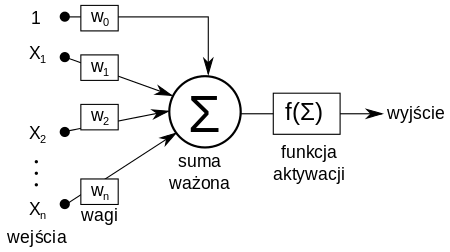
\includegraphics[angle=0, width=0.45\textwidth]{Model Neuronu.png}
\caption{Model neuronu Mcculocha-Pittsa \cite{MC-P-wiki}}
\end{center}
\end{figure}

Neuron jest połączony tu z neuronami presynaptycznymi. Pobiera z nich ich stan wzbudzenia oraz mnoży tą wartość przez siłę połąćzenia danej pary neuronów. Następnie wartości te są sumowane do jednej wartości a w kolejnym kroku przetwarzamy otrzymaną liczbę funkcją aktywacji. Dopiero tak przetworzona liczba jest końcowym stanem aktywacji neuronu.


\subsection{Głębokie sieci neuronowe}
Kolejnym krokiem będzie połączenie tych neuronów w sieć, która to będzie zdolna do przetwarzania sygnałów wejściowych. W sieci neuronowej możemy wydzielić 3 typy warstw. Warstwę wejściową, nieposiadającą żadnych neuronów presynaptycznych, których stan aktywacji uzależniamy od danych wejściowych. Warstwe ukrytą. Warstwe wyjściową, której stan wyjściowy pobieramy, interpretujemy oraz decydujemy jaką podjąć akcję w danej sytuacji.

Głębokie sieci neuronowe - jest to model matematyczny, którego działanie ma symulować sposób działania biologicznych seici neuronowych.

\subsection{Reprezentacja matemamtyczna}
Operacje przeprowadzane na sieci, można zamodelować przez macierze. Wystarczy zauważyć, że sygnał wejściowy do każdej warstwy można zapisać przy pomocy wektora, oraz każdą warstwe charakteryzuje macierz, gdzie w każdym wierszu znajdują się wagi połączeń dla neurowanów z roważanej wartwy. Wtedy możemy zamodelować przejście sygnału przez warstwę równaniem.

\begin{equation}
    X_{1 \times N}' = f(X_{1 \times M}*A_{M \times N} + B_{1 \times N})
\end{equation}

Operacja ta może zostać wykoanana na każdej warstwie, dzięki czemu uzyskujemy stosunkowo szybki sposób na ewaluacje danego zbioru danych.

\subsection{Wsteczna propagacja}
Wsteczna propagacja jest sposobem uczenia sieci. Jej działanie jest dużo bardziej złożone w stosunku do obliczenia wartości "do przodu". Metoda ta polega na tym, iż usykujemy pewną informacje zwrotną jak dobrze sieć jest aktualnie wytrenowana. Aby uzyskać taką ewaluacje, możemy albo użyć pewnej funckji nagrody albo pewnego zestawu informacji, których znamy poprawną ewaluacje. Przy jednym jak i drugim uzsykujemy możemy uzyskać informacje jak dobrze sobie aktualnie radzi sieć.

\begin{equation}
    X_{1 \times N}' = f(X_{1 \times M}*A_{M \times N} + B_{1 \times N})
\end{equation}



\section{Wykonanie}

\section{Bibliografia}

\begin{thebibliography}{9}


\bibitem{MC-P-wiki}
    https://pl.wikipedia.org/wiki/Neuron\_McCullocha-Pittsa

\bibitem{lamport94}
  Leslie Lamport,
  \emph{\LaTeX: A Document Preparation System}.
  Addison Wesley, Massachusetts,
  2nd Edition,
  1994.

\end{thebibliography}

\end{document}
